Consider the following feedback system.
\begin{center}
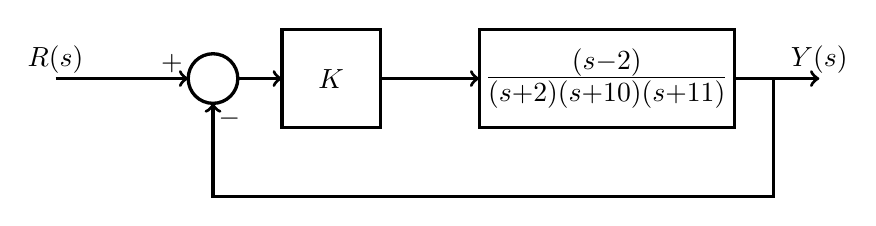
\begin{tikzpicture}[scale=1,inner sep=0pt,outer sep=0pt,very thick,
sysblock/.style={draw,rectangle,inner sep=2pt,minimum width=1.25cm,minimum height=1.25cm,very thick}]
\draw (2,0) node[draw,circle] (sum1) {$\rule{0pt}{18pt}$};
\draw (3.5,0) node[sysblock] (Kp) {$ K$};
\draw (7,0) node[sysblock] (G) {\Large $\frac{(s-2)}{(s+2)(s+10)(s+11)}$};
\draw[->] (0,0) node[above=2pt] {$R(s)$} -- (sum1.180) node[above left=2pt] {$+$};
\draw[->] (sum1.0) --  (Kp);
\draw[->] (Kp) -- (G);
\draw[->] (G) -- ++(2.7,0) node[above=2pt] {$Y(s)$};
\draw[->] (G.0) ++(.5,0) -- ++(0,-1.5) -| (sum1.-90) node[below right=2pt] {$-$};
\end{tikzpicture}
\end{center}
\begin{enumerate}[(a)]
\item Sketch the root locus of closed loop poles for varying $K$. 
\item On your sketch, indicate the region where the closed loop poles will satisfy the step response specification of settling time $t_{s}<4.6$s. 
\item Does there exist a $K$ such that the dominant pole or poles of the closed loop system would satisfy this requirement?
\end{enumerate}
